  \chapter{Introduction}\label{chp1_intro}
\objectif{On universality in population genetics}

%%%%%%%%%%%%%%%%%%%%%%%%%%%%%%%%%%%%%%%%%%%%%%%%%%%%%%%%%%%%%%%%%%%%%%%%%%%%%%%%%%%%%%%%%%%%%%%%%


\section{Modeling complex populations with simple objects}

Population genetics studies how the genetic composition of a population changes
over generations under the combined effect of reproduction, random sampling and selection. 
The origins of discipline traces back to the early 19th century, when Lamarck~\cite{de_monet_de_lamarck_philosophie_1809} proposed one of the first theories of evolution, based on the inheritance of characteristics acquired during an organism's lifetime. 20 years later, Darwin developed a different explanation after an expedition in South America during which he observed the diversity of species and their geographical variation. In the late 1830s, he formulated the theory of natural selection as the main driver of the transformation and diversification of species~\cite{darwin_origin_1859}. 

In the 1960s, Motoo Kimura~\cite{kimura_evolutionary_1968} argued that the vast majority of mutations are neutral. According to this view, the genetic diversity observed in nature is shaped mainly by chance rather than by Darwinian natural selection. As a consequence, variation at the molecular level is governed by \emph{genetic drift}, which refers to the random change in the frequency of an allele in a population from one generation to the next.
The central question, which sparked a big controversy at the time, was the following:\\
\\
\emph{Can we explain all the observed polymorphism in natural populations without needing to invoke natural selection?}
\\
\\
This was the beginning of the so-call \textit{neutral theory of molecular evolution}, which provides the evolutionary framework on which many of the models used today are based.

The simplest setting in which this question can be posed
rigorously is that of a \emph{well-mixed} population with fixed size and in which every individual is, at each generation, equally likely to be the parent of any other individual. This model is called the Wright--Fisher model~\citep{wright_evolution_1931,fisher_genetical_1930} and serves as the basis to Kimura's neutral theory~\cite{kimura_evolutionary_1968}. 

This section recalls the classical descriptions of neutral, purely conservative population models, forward in time through models of reproduction, and backward in time through genealogies, and the universal objects, the Wright-Fisher diffusion
and the Kingman coalescent, that these descriptions converge to in the large population limit.
\paragraph{Notations.}
Throughout this work, we denote by $K$ a large demographic parameter that represents the size (or the order of magnitude of the size) of a population. For both discrete and continuous time models, we will denote by $t$ the time index, which can be either discrete or continuous. We will denote by $\mathcal{N}_t$ the set of individuals in the population at time $t$. The letter $z$ will refer to a notion of density (either allele frequencies or population densities in regulated models). 
\subsection{Discrete neutral population models}\label{sec:neutral_models}
\paragraph{Exchangeable models in discrete time.} Tracing back to the 1930 with the work of Wright~\cite{wright_evolution_1931} and Fisher~\cite{fisher_genetical_1930},
 the Wright-Fisher model is a stochastic model used as a baseline in evolutionary biology, population genetics and phylogenetics. It models the development of genetic variability within a population, explaining the genetic drift. In its simplest form, consider a population of $K$ individuals labeled $1,\dots,K$, each carrying one of two alleles, $A$ or $a$. The population is assumed to be well-mixed, meaning that every individual is equally likely to mate with any other individual. The model assumes discrete generations, where each generation is formed by sampling uniformly at random and with replacement a parent from the previous generation.

 An important assumption made here is the notion of \emph{exchangeability}: the law of the model vector is invariant under permutation of the labels of the individuals. Moreover, it is independent and identically distributed
across generations. 


 More generally, Cannings models~\cite{cannings_latent_1974,cannings_latent_1975} denote the family of discrete-generation, exchangeable population frameworks that generalize classical genetic models.
Fix $K \ge 2$. In the Cannings model, generations are indexed by $t \in \mathbb K$,
and each generation consists of $K$ individuals, labelled $1,\dots,K$. Individual
$i$ in generation $t$ produces $\nu_i(t) \ge 0$ offspring in generation $t+1$, and the progeny inherit the allele of their parent.

The offspring vector is denoted by
\[
\nu(t)\ \coloneqq\ (\nu_1(t),\dots,\nu_K(t)),\quad \text{such that}\quad \sum_{i=1}^K \nu_i(t)\ =\ K.
\] 
Cannings models is the most general class of neutral, exchangeable reproduction schemes with
fixed population size and non-overlapping generations, in the sense that no
further assumption is made on the offspring distribution beyond exchangeability
and the constraint $\sum_i \nu_i(t) = K$. The Wright-Fisher model is a particular instance of Cannings models, which corresponds to choosing the vector 
$\nu(t)$ to be distributed as a multinomial random vector:
\[
\forall t\in \N,\quad \nu(t)\ \sim\ \mathrm{multinom}(K; 1/K,\dots,1/K).
\]

\paragraph{Continuous-time exchangeable models.} 
Biological problems are usually modeled as continuous-time phenomena. 
The continuous-time analogue of the Wright-Fisher model is the Moran model. This is a continuous-time Markov chain in which individuals reproduce at independent exponential times, and each offspring replaces a uniformly chosen individual in the population. 

The Moran model extends naturally to non-binary reproduction events, in which a single individual can produce multiple offspring at once, replacing a random number of individuals in the population.  This model has been studied for instance in~\citet{etheridge_coalescent_2010,birkner_measure-valued_2009}. The evolution of the population is given by a resampling mechanism: each $d$-uplet of individuals dies after an exponential holding time with some positive rate $\lambda_d$. Upon death, one individual of the $d$-uplet is replaced by $d$ copies of themselves. This is called the $\Lambda$-Moran model.


\subsection{Universal scaling limits}
We introduce the two universal objects that emerge as scaling limits of the idealized discrete-time models presented in the previous section, and that will be used throughout this thesis.
\paragraph{Prospective limit: the Wright--Fisher diffusion.}
When the population size goes to infinity, the evolution of the frequency of a given allele in the Wright-Fisher model converges to a continuous-time, Gaussian object called the Wright-Fisher diffusion. It is a diffusion process on the unit interval $[0,1]$ that is the weak solution to the stochastic differential equation
\[
dZ_t\ =\ \sqrt{Z_t(1-Z_t)} dB_t,
\]
where $B_t$ is a standard Brownian motion. In an equivalent manner, the Wright--Fisher diffusion is described by its infinitesimal generator, which acts on twice continuously differentiable functions $f:[0,1]\to \R$ as
\[
\mathcal{G}_{WF} f(x)\ =\ \frac{1}{2} x(1-x) f''(x),\quad x\ \in\ [0,1].
\]
The Wright-Fisher diffusion is the scaling limit of the Moran model as well, and more generally of any Cannings model with finite offspring variance.

More generally, if we track the frequency of $k\geq 2$ neutral alleles in a population, then the joint evolution of the frequencies of these alleles (which we will refer to as \emph{neutral fractions} in Chapter~\ref{chp4_multitype}) is described in the large population limit by a diffusion process on the $k$-dimensional simplex $\Delta^{k}=\{x\in[0,1]^{k}:\sum_{i=1}^{k}x_i = 1\}$ called the $k$-allele Wright-Fisher diffusion. It is characterized by its infinitesimal generator, which acts on twice continuously differentiable functions $f:\R^{k}\to \R$ as
\[
 \mathcal{G}^k_{WF} f(\bm x)\ =\ \frac{1}{2}\sum_{i,j=1}^k x_i(\delta_{ij}-x_j) \partial_{i,j}f(\bm x), \quad \bm x\ =\ (x_1,\dots,x_k)\ \in\ \Delta^k.
\]

Adding selection to Cannings model with finite variance leads to a drift term in the Wright-Fisher diffusion, while modifying the variance of the offspring distribution changes the diffusion coefficient. 
\paragraph{Retrospective limit: neutral coalescent theory.}
An alternative way to describe the allelic composition of a population is to
sample individuals uniformly from the population at some fixed ``present'' time $t$, and to trace their ancestral relationships backward in time, locating the most recent common ancestor. 
This backward-in-time approach is called coalescent theory.
Tracking the ancestral lineages yields an (ultra)metric structure on the space of individuals alive at time $t$, equipped with the following \emph{genetic distance}
Fix $t>0$ and $k\geq 1$. We recall that ${\cal N}_t$ denotes the set of individuals alive at time $t$.
For any pair $u,v \in{\cal N}_t$ with $u\neq v$, we denote
by $D_{t}(u, v)$  the genetic distance between $u$ and $v$,  defined as the time to the death of their most recent common ancestor, see Figure~\ref{fig:distance_gen_intro}.

\begin{figure}[h!]
    \centering
\resizebox{0.6\textwidth}{!}{
\begin{tikzpicture}[x=0.75pt,y=0.75pt,yscale=-1,xscale=1]
%uncomment if require: \path (0,200); %set diagram left start at 0, and has height of 200

%Image [id:dp5479612406703641] 
\draw (295.5,90.03) node  {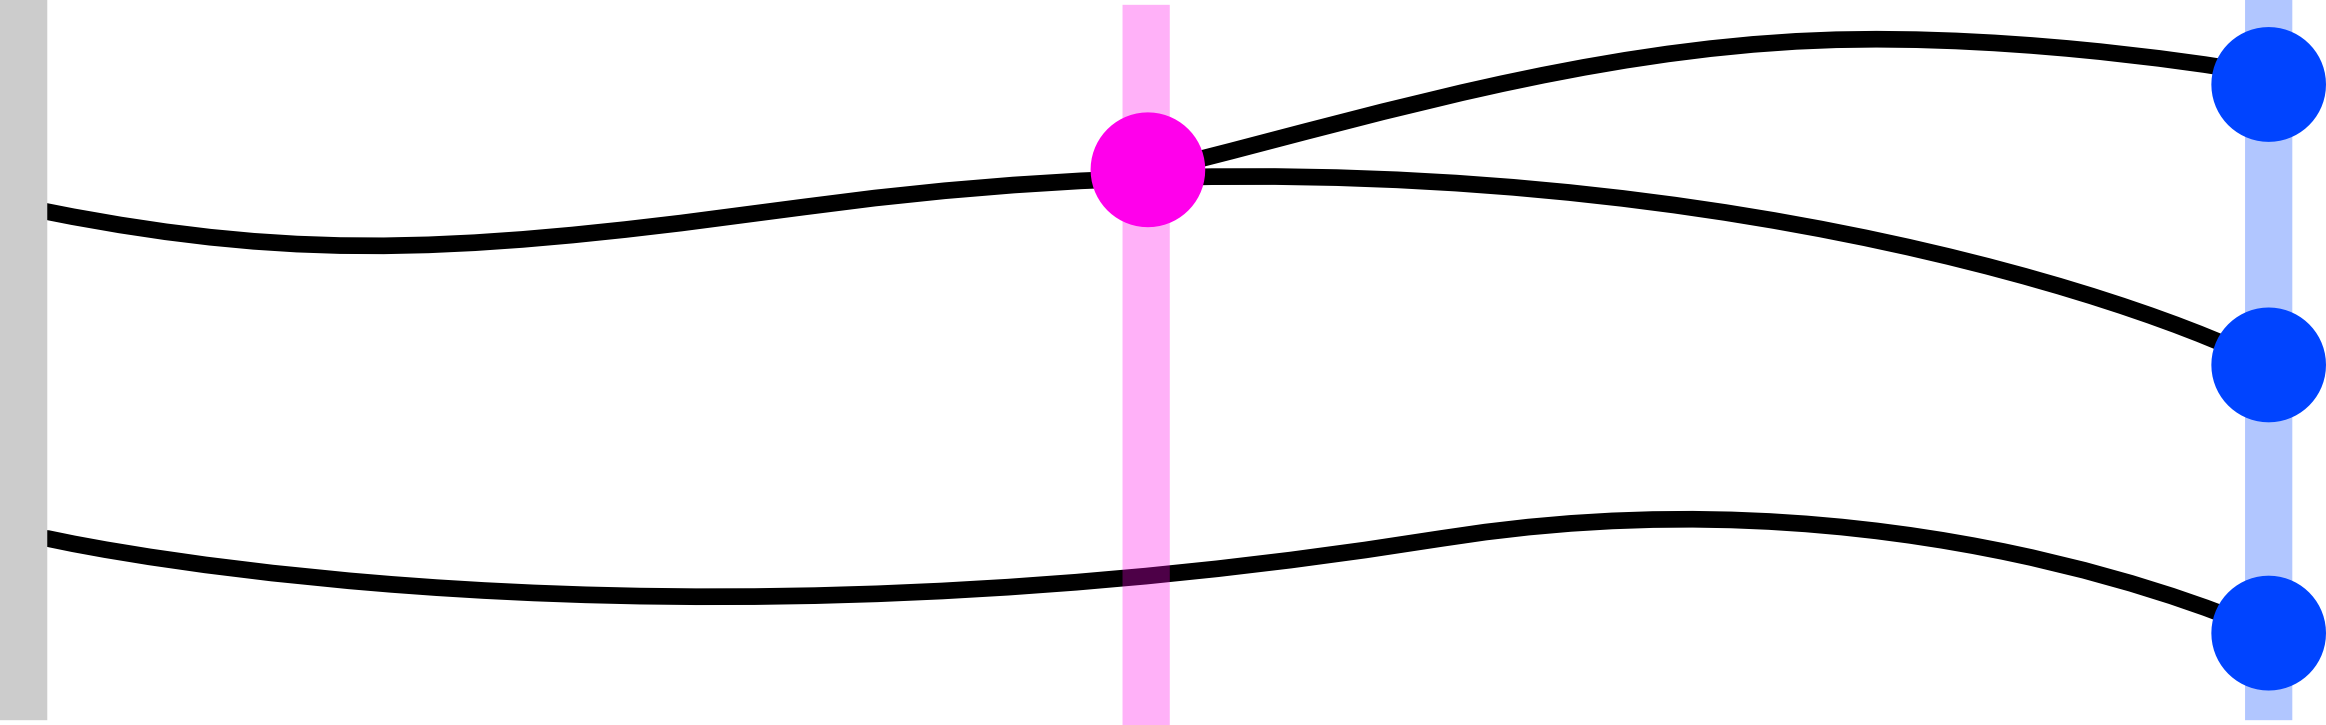
\includegraphics[width=440.25pt,height=132.05pt]{ch4/fig/distance_gen.png}};

% Text Node
\draw (4,181.46) node [anchor=north west][inner sep=0.75pt]    {\Large $s=\ 0\ =\ t-D_{t}( u,w)$};
% Text Node
\draw (285,180.46) node [anchor=north west][inner sep=0.75pt]    {\Large $s=t-D_{t}( u,v)$};
% Text Node
\draw (570,180.46) node [anchor=north west][inner sep=0.75pt]    {\Large $s=t$};
% Text Node
\draw (597,13.4) node [anchor=north west][inner sep=0.75pt]    {\Large $u$};
% Text Node
\draw (596,82.4) node [anchor=north west][inner sep=0.75pt]    {\Large $v$};
% Text Node
\draw (595,150.4) node [anchor=north west][inner sep=0.75pt]    {\Large $w$};

\end{tikzpicture}}
    \caption{Genealogical distances between individuals $u,v,w\in {\cal N}_t$. The pink particle is the most recent common ancestor of $u$ and $v$.}
    \label{fig:distance_gen_intro}
\end{figure}

%In the case  
%$u=v$, we set $D_{KT}(u, u) = 0$. 
Conditional on the event $\{|{\cal N}_t|\geq k\}$, let 
$(U_1, \dots, U_k)$ be $k\geq 1$ individuals
sampled uniformly \emph{without replacement} from ${\cal N}_t$.

We introduce the process
$({\cal C}^{k}_{s,t})_{s \in [0, t]}$ with values in the partitions of
$\{1,\dots, k\}$ satisfying that
\[
    \forall \tau\leq t, \ \ i \sim_{{\cal C}^{k}_{s,t}} j\ \iff\
  D_{t}(U_i, U_j)\ \leq\  s.
\]
This partition-valued process encodes the subforest spanned by the sample $(U_i)_{i \leq k}$. 


In neutral models of population genetics, the standard statement is the following:
conditional on a genealogy, neutral mutations are superimposed independently on its branches according to Poisson processes with rate proportional to the branches' length~\cite{donnelly_coalescents_1995, griffiths_genealogy_2003}. 
Thus, the shape of the genealogies determines how many mutations we see and how frequent they are. Long branches imply more diversity, while shallow branching points imply that many individuals share a recent common ancestor, which in turn means that there is low diversity in the population. 
\medskip

\paragraph{Exchangeable coalescents.}
In particular, the limiting genealogy of the Moran Model is described by a continuous-time Markov chain on the space of partitions of $\{1,\ldots,n\}$ called the Kingman coalescent. It was introduced by Kingman in 1982~\cite{Kingman:1982aa}.

The Kingman coalescent with rate $r$ is the partition-valued process started from the singleton partition and such that each pair of blocks merge at rate $r$. 
Thus, the block-counting process is the decreasing integer-valued process with transitions
\[
n\ \longrightarrow\ n-1 \qquad \text{at rate}\quad r\binom{n}{2}.
\]

The pairwise merging rate is linked to the scaling limit of the variance of the forward in time Wright--Fisher model through the formula
\[
r\ =\  \E\big[\nu_1(t)(\nu_1(t)-1)\big].
\]
The genetic diversity of the population is captured by this pairwise merging rate of the coalescent, and thus to the variance of the offspring distribution in the forward-in-time model. We will develop this notion of  \emph{effective population size} in the next section. 


However, if the variance of the offspring distribution is infinite, then the Kingman coalescent can no longer be a good estimate for the genealogies of the population. Notably, we say that a probability distribution $L$ with values in $\R_+$ is heavy-tailed if its tail probability $\Prob(L > x)$ decays slower than any exponential as $x\to\infty$

In particular, it has a power-law tail if there exists $\alpha \in (1,2)$ such that
\[
\Prob(L > x)\ \sim\ C x^{-\alpha} \quad \textit{as}\quad x\ \to\ \infty.
\]

If the offspring distribution per individual in a Cannings model is heavy-tailed, then a single individual can, with non-negligible probability, produce a positive fraction of the whole next generation.
Zooming out, these large birth events create big families who persist in the large population limit. Looking at the genealogies, individuals at present are likely to descend from these large families, so that the diversity of the population is reduced and the genealogy of the population is no longer described by a binary tree like the Kingman coalescent, but rather by a tree with multiple mergers. 

Pitman~\cite{Pitman:1999aa} and Sagitov~\cite{sagitov1999general} characterized the class of exchangeable coalescent processes admitting multiple mergers. That is, merging events involving several blocks, but at most one merger event at a time. Given a finite measure $\Lambda$ on $[0,1]$, the $\Lambda$-coalescent is the Markov chain on the space of partitions of $\{1,\ldots,n\}$ with the following dynamics:
 Starting from the singleton partition, if there are $b$ blocks present, any given group of $k$ of them $(2 \leq k \leq b)$ merges into one at rate
\[
\lambda_{b,k}\ =\ \int_0^1 x^{k-2} (1-x)^{b-k}\, \Lambda(dx),
\]
independently of the other groups.  Taking $\Lambda = \delta_0$ in the above display recovers the Kingman coalescent. In the beginning of the century, Möhle and Sagitov~\cite{mohle_classification_2001,Mohle_Sagitov} provided the exact conditions on the offspring distribution of a Cannings model under which its genealogy, once suitably rescaled, converges to a $\Lambda$-coalescent. 
In particular, if the law of $\nu_1$ has a power tail with parameter $\alpha$, then the genealogies converge to a $\Lambda$-coalescent with measure $\Lambda=\mathrm{Beta}(1-\alpha, \alpha)$.
Thereby, they classified the possible scaling limits of the genealogies in exchangeable populations with fixed size.

\paragraph{Duality}
The Wright--Fisher diffusion and the Kingman coalescent can be seen as being two sides of the same coin: both describe a scaling limit in the Moran and Wright--Fisher population models, respectively forward and backward-in-time. More generally, if the neutral fractions in a population model are shown to converge forward-in-time to the Wright--Fisher diffusion, it is expected for the genealogies to converge to the Kingman coalescent, and if they converge to a $\Lambda$-Fleming--Viot, then the genealogies should converge to exchangeable coalescent with multiple merges. This heuristic has been rigorously established only within certain classes of models, such as Cannings models~\cite{mohle_convergence_1998,Mohle_Sagitov}.

The forward and backward descriptions of neutral exchangeable populations are linked by a \emph{moment duality} formula. 
Duality is a fundamental concept in mathematics and takes different forms. The underlying idea is to control a complex object by using a simpler one, which potentially takes values in a different space.  

When it comes to population models, Markovian duality is a powerful tool to connect two stochastic processes. In particular, it often relates the forward-in-time evolution of allele frequencies  to a backward-in-time process describing genealogical quantities, for example the number of ancestral lineages. The moment duality between Wright-Fisher diffusion and Kingman's coalescent is certainly the most famous instance of duality in population genetics.
Denote by 
$X_t \in [0,1]$ the frequency of an allele at time $t$ in the Wright--Fisher diffusion, and by $N(t)$ the number of blocks in the Kingman coalescent
 Then, we have
\[
\E_{x}\big[X_t^{n}\big]\ =\ \E_n\big[x^{ N(t)}\big].
\]
 We refer to \cite{etheridge_mathematical_2011,ethier_1986, mohle_concept_1999, carinci_dualities_2015, cordero_bernstein_2026, blath_separation_2021,etheridge_coalescent_2010} for other forms of dualities in population genetics.

However, there is no general method allowing us to deduce the formal distribution of the coalescent directly from the forward-in-time dynamics. For most models, as highlighted in~\cite{Julie_Zsofia}, it remains a technical challenge.
 
\section{Central questions in applied population genetics}

\subsection{Lewontin's paradox and the effective population size}


Genetic drift was demonstrated experimentally in the PhD thesis of Buri~\cite{buri_gene_1956}, who followed populations of \emph{Drosophila melanogaster}. Over 19 generations, allele frequencies drifted randomly, and many populations ended up fixed for one allele or the other. Importantly, the observed loss of heterozygosity was faster than predicted by the Wright--Fisher model for random. This means that the populations behaved as if they were smaller. This result illustrates a great paradox in population genetics.

\paragraph{Lewontin's paradox of genetic diversity}
Neutral theory and the class of unstructured exchangeable models assume that in a population of size $N$, diversity results from an equilibrium between new mutations arising at a constant rate $\mu$ and genetic drift that purge them at a rate $1/N$. Thus, according to neutral models, the predicted quantitative  value for genetic diversity at equilibrium should be proportional to $N\mu$. The discrepancy between the neutralist's expectation and the much lower observed levels of genetic diversity in real populations is known as the Lewontin paradox~\cite{lewontin_genetic_1974, leffler_revisiting_2012}.


\paragraph{The effective population size}
Wright \cite{wright_evolution_1931} proposed to account for such discrepancies, and more generally for any departure from the idealized Wright-Fisher setting, by
introducing an \emph{effective population size}, which is classically denoted by $N_e$ in the litterature.
The effective Population Size captures the number of individuals that effectively participates in producing the next generation. It reflects how much genetic drift a real population experiences, hence its rate of loss of genetic variability. It accounts for parameters such as demographic fluctuations, variance in reproductive success, population structure, sex ratio, linked selection, etc. These parameters greatly influence evolutionary processes.
 Generally, the effective size of a population is considerably less than its census size,  with a $1:1$ ratio only in the special case of an ``ideal'' panmictic population, in which variation among individuals in reproductive success is completely random. 

Lewontin's paradox illustrates why the effective population size, rather than the number of individuals, is the relevant quantity in evolutionary biology for understanding genetic diversity (even if it should be pointed out that $N_e$ is not sufficient to resolve the paradox, as can be seen \eg in~\citet{buffalo_quantifying_2021}). It has been widely used across scientific fields and has received considerable attention over the past decades. Estimating $N_e$ is crucial for conservation and biodiversity monitoring, \eg to classify and protect endangered species. Populations with low genetic diversity are more vulnerable to disease, climate change, and other stressors, and may be at risk of extinction even when their census size is large~\cite{mergeay_importance_2026, frankham_effective_1995}.
However, it does not have a universal and constant in time definition: it was initially introduced in the 1930s by Sewall Wright~\cite{wright_evolution_1931} as follows:
\\
\\
\textit{
  ``The number of surviving offspring left by different parents may vary tremendously either through selection or merely accidental causes, a condition which tends to reduce the effective N far below the actual number of parents or even of grandparents.''
}--\citet{wright_evolution_1931}
\\
\\
From this definition, $N_e$ is the size of an idealized well-mixed Wright--Fisher population whose rate of genetic drift, measured for instance by the pairwise coalescence time or by the rate of loss of heterozygosity, matches that of the population under study. 

Several, non-equivalent, definitions of $N_e$ have since been developed. 
For example, using the change of inbreeding (see~\citet{crow_inbreeding_1988}), the variance in reproductive success, 
the coalescent rate of lineages backward in time (see~\citet{Kingman:1982aa}), the linkage disequilibrium (that is, the nonrandom association between alleles at different loci~\cite{slatkin_linkage_2008}), the sibling relationships among sampled individuals, etc.
We refer to Charlesworth~\cite{charlesworth_effective_2009,charlesworth_how_2022} and Waples~\cite{waples_what_2022,waples_idiots_2025} for reviews over the different definitions of this concept. To each definition of $N_e$ corresponds a principle of inferring it.
In Chapter~\ref{chp3_singletype} and Chapter~\ref{chp4_multitype} of this thesis, we will use the definition of $N_e$ that relates to coalescent theory: the pairwise merging rate $r$ of linages in a Kingman coalescent relates to the effective population size through
\[
r\ =\ \frac{1}{N_e}.
\]

\subsection{Neutral models in practice}
Neutral models and the whole class of unstructured, exchangeable models presented in the last paragraphs all rest on idealizations, constant population size, panmixia and neutrality of reproduction. Essentially, no natural population satisfies these assumptions exactly.


In applied population genetics, the neutral theory is the principal inferential tool.

\paragraph{Inferring genealogies from data}
\begin{itemize}
\item Site-Frequency spectrum (SFS): tells something about the shape of the tree but not on the length of the branches
\item \cite{griffiths_ancestral_2001} outlines statistical and coalescent methods to reconstruct the evolutionary history of DNA sequences.
\end{itemize}

In particular, phylodynamics treats the Kingman coalescent as the default tree-generating model to reconstruct a phylogeny from sampled gene sequences. Inverting it allows to infer the demographic history of a population according to the following observation: 
Under the Kingman coalescent, if during the $i^{th}$ inter-coalescence interval, $n_i$ lineages are present, then the expected length of the interval is $N_e(t)/\binom{n_i}{2}$. The effective population size at time $t$ can be read directly off the observed branch lengths of the tree (see figure~\ref{fig:skyline_plot}). This method is called the \emph{skyline plot} and was introduced by \cite{pybus_integrated_2000}. This method, and its Bayesian variants, is used routinely to reconstruct the demographic history of viral epidemics and other rapidly evolving pathogens \citep{pybus_evolutionary_2009,ho_skyline-plot_2011}, none of which reproduce according to literal Wright-Fisher dynamics. It works because, as recalled above, the Kingman coalescent is the common scaling limit of every Cannings model with finite offspring variance, so the $N_e$ it returns remains a meaningful summary of genetic diversity regardless of the true, unknown reproduction mechanism within the population. 

\begin{figure}[h!]
    \centering
\includegraphics[width=0.5\textwidth]{intro/fig/skyline_plot.pdf}
\caption{Reconstruction of the tree from the Skyline plot, figure from~\cite{ho_skyline-plot_2011}}
\label{fig:skyline_plot}
\end{figure}
The approach breaks down when reproduction is itself strongly skewed, epidemic superspreading, selective sweeps, oversampling, which produce multifurcating genealogies that the almost surely binary Kingman coalescent cannot generate; here it is again a simple, exchangeable model, the $\Lambda$-coalescent, that is used to extend the skyline plot and recover the ability to infer demographic history \citep{hoscheit_multifurcating_2019}. 


Exchangeable coalescents (Kingman, $\Lambda$-coalescents) and neutral models are the standard null hypothesis for modeling complex populations.
Yet, does it still make sense to use these processes to explain genetics diversity in the wild? The answer given by mathematics is broadly positive. 

On the theoretical side, the Kingman's coalescent has been proved to be robust to modifications from the tight assumptions of the Wright--Fisher model, and arises as the genealogy of a broad class of forward-in-time population models. Beyond the purely neutral setting presented in Section~\ref{sec:neutral_models}, the Kingman coalescent process has served as the backbone onto which further biological ingredients are grafted. For instance, variation of population size over time is incorporated by a deterministic time change of the coalescent rate
\citep{griffiths_sampling_1994, Jagers2004ConvergenceTT}, or by a stochastic time change in models with stochastically varying population size~\cite{kaj_coalescent_2003}.
Exchangeable coalescents also appear as the limiting genealogies of population models with selection \citep{kaplan_coalescent_1988, neuhauser_genealogy_1997}, recombination \citep{hudson_coalescent_1988}, diploid biparental models \citep{wakeley_gene_2012, koskela_robust_2019}, non-excheangeable models~\citep{siri-jegousse_exchangeable_2024}, etc. 
We also refer to~\cite{Brown:2023aa} for non-neutral models converging to the Kingman coalescent.

\paragraph{Motivation of the PhD thesis.}
We saw that, after a suitable scaling, the Wright--Fisher diffusion and the Kingman coalescent appear as the (forward and backward) scaling limits of Cannings models with finite variance and selection. 

Here, we can draw a parallel between the Wright-Fisher diffusion and other Gaussian objects that are universal scaling limits in probability. The simplest instance is that of \iid Bernoulli experiments. The rescaled number of heads in a sequence of perfect coin tosses converges to a Gaussian random variable. Variation of this experiment, for instance by adding a bias to the coin, leads to a re-scaling of the same object by a drift term. Likewise, it is well established by Donsker's theorem that the Brownian motion is the universal scaling limit of random walks with finite variance. The symmetric random walk converges to the standard Brownian motion, while other random walks with finite variance converge to a rescaling of this universal Gaussian object.


In the same way, current research works show that the Wright-Fisher diffusion and the Kingman coalescent are the universal scaling limit of neutral populations with finite variance. Population with skewed reproduction, in which a single individual can produce a positive fraction of the next generation, converge to a different class of universal objects, the $\Lambda$-Wright-Fisher diffusion and $\Lambda$-coalescents.

In light of the preceding paragraph, this thesis is motivated by a single conjecture about universality in population genetics:
\\

\emph{Large populations that are structured and regulated become indistinguishable from a well-mixed Wright--Fisher population, provided the parameters are suitably rescaled. Two quantities carry this rescaling: an effective population size $N_e$, and an effective selection coefficient $s_e$, which captures how the interplay of structure, regulation, and selection alters the fate of an allele.
}
\\

Our aim in Chapter~\ref{chp3_singletype} and~\ref{chp4_multitype} is to move toward this statement and to identify general conditions under which the genetic diversity of a population can be described by a rescaling of neutral models, even when its ecology is complex. Specifically, we ask when a structured, interacting population still behaves on the coalescent timescale as though it were well mixed, with some effective size $N_e$.

\section{Understanding the play of ecology in genetic diversity}
A lot of recent research works indicate that not taking into account the structure of a population seriously misrepresents the estimate of changes in effective population size over time, and thus of the population's genetic diversity. If ecology is not taken into account, a structured population can thus mimic the genetic signature of a population decline (bottleneck) or a completely fictitious event of interbreeding (see~\citet{mazet_importance_2016}). 

Movement of population can take several forms across species. For example, one can think of the seasonal migrations observed in some populations, in particular within birds (barnacle geese, storks, but also salmons). Movement can also be initiated by density-denpendent competition and the need to explore new inhabitats in search of resources. 

Within interacting populations, the homogeneization principle allowing to describe the population using neutral models and some effective parameters is only established in
full generality for a very restricted class of models called \emph{meta-population} models. Extending these results to more involved structured models presents notable challenges.
\subsection{State of the art: meta-populations models}
Meta-population models refer to models of population with constant size (hence no demography) and a finite type structure. We give a few examples of such celebrated models, and refer to~\citet{etheridge_mathematical_2011} for a broader review.
 
\paragraph{Prospective picture: island models}
Wright-Fisher with migration: Wright's island model \cite{wright_isolation_1943} (migration on the complete graph or $\Z^2$, discrete approximation of spatially structured models)
Stepping-stone models:
Diffusion approximation in each deme~\cite{kimura_stepping_1964}
As in the monotype Cannings model, the population size is fixed on each site. Thus, a birth on one site has to coincide with a death on another
site.
\paragraph{Retrospective picture: the structured coalescent}
The genealogical counterpart of the stepping-stone and island models is the
structured coalescent: lineages ancestral to a sample coalesce, at rate
depending on the local deme size, only when they occupy the same deme, and
migrate between demes according to the time-reversal of the forward migration
mechanism. Nordborg and Krone \cite{nordborg_separation_2002} study the
conditions under which this process, once demes and migration rates are held
fixed and time is suitably rescaled, converges to an unstructured coalescent.
The structured coalescent is dual, in the sense of Section 1.2, to the
forward-in-time stepping-stone model \cite[Chapter~4]{etheridge_mathematical_2011}.
This duality extends to Cannings-type reproduction within each deme, yielding
multitype exchangeable coalescents in which the deme sizes are themselves random
\cite{huillet_asymptotic_2021,mohle_multi-type_2024}.



\paragraph{Universality, collapse of the structure}
\cite{nordborg_separation_2002}: effective coalescence rate in fast migration regime, decorellation of timescales.
\cite{zahle_stepping_2005}
\cite{nagylaki_strong-migration_1980}: strong migration regime
\cite{wilkinson-herbots_coalescence_2003}: Conditions on the graph structure to guarantee convergence to the neutral coalescent independently of the migration pattern.
\cite{Julie_Zsofia} (neutral fractions)

\subsection{Regulated populations in finite type spaces}
Meta-population models are very restrictive when it comes to describing real populations. In particular, we observe that there is no demography: the population size is fixed, so that reproduction events of individuals are anti-correlated.


When it comes to structured, interacting population models that allows for demography, the picture for the ancestral lineages is less clear. In the countable type space setting,~\cite{Bansaye} studied an individual-based model with density-dependent interaction, and retrieved 
the empirical distribution of the types along a typical surviving lineage.
The connection between neutral fractions and ancestral lineages was also used in \citet{forien_ancestral_2022} to study genealogies in a one dimensional PDE model with competition and selection, adapting to a moving environmental optimum.
An individual-based model version of the SDE model of~\cite{forien_ancestral_2022} was studied in~\cite{meleard-tran}. They obtained the convergence of the typical ancestral type trajectory to an Ornstein--Uhlenbeck process, using a many-to-one formula. 
 Genealogies of interacting particle systems have been studied in many specific models using other methods, for instance we cite~\cite{alison_m_etheridge_looking_2024} where the authors used a lookdown construction to derive the genealogy of a birth-death process in a spatial structure, regulated by local interactions. We also point out \cite{etheridge_genealogies_2022} who studied a diploid individual-based spatial (one dimensional) Moran model with interactions and cooperation (allee effect). They proved using a heuristic that the genealogy of the model converges to a Kingman coalescent.
\paragraph{Density dependence and constrained populations}

\ma{describe model and assumptions}

In this framework,~\cite{Kurtz:1978aa} established a law of large number for the rescaled count of types in the population, under regularity assumptions 
\begin{prop}{\citet[Theorem~2.2]{Kurtz:1978aa}}
  Assume that $\lim_{K\to\infty}Z_0\eqqcolon z_0$ exists almost-surely in $\R_+^E$ and denote by
  $(z_t)_{t\geq 0}$ the solution to the $E$-dimensional dynamical system 
  \begin{equation*}
\dot z_t\ =\ z_t M(z_t),
\end{equation*}
with initial condition $z_0$.
Assume that $z\mapsto zM(z)$ is Lipchitz and that for all $n\in\N^E$, $\exists\ C_n>0$ such that $\sum_n \lVert n\rVert C_n<\infty$ and
\[
\sup_{x\in E, z\in \R_+^E} z_x q_x(z) \Prob(L_x(z)=n)\ \leq\ C_n(1+ \lVert z\rVert).
\]
Then the limit
\[
\adjustlimits{\lim}_{K\to\infty}{\sup}_{t\leq T} \big|Z_t-z_t\big| \ \longrightarrow\ 0
\]
holds in probability, for every $T>0$.
\end{prop}
Moreover, under additional assumptions on the offspring distribution, Kurtz also established a central limit theorem for the fluctuations of the rescaled count of types around the deterministic limit. In particular, he showed that these fluctuations converge to an Ornstein--Uhlenbeck process (see \cite[Theorem 4.4]{Kurtz:1978aa}), at a speed $\sqrt{K}$.

\cite{etheridge_genealogies_2022}

\subsection{Continuous models}
Wright-Malécot (models in $\R$ and $\R^2$)
\cite{nagylaki_diffusion_1978}: Diffusion model on an unbounded linear type space, derived a relation for correlations between allele frequencies at different locations, but fails in $\R^2$
\paragraph{The spatial $\Lambda$-Flemning--Viot Process.}
\cite{barton_new_2010}: Genealogy to a sample can be described in
terms of a spatial version of the $\Lambda$-coalescent. There is convergence of ancestral lineages to the Kingman coalescent or the non-spatial $\Lambda$-coalescent in some regime of parameters (detailed in \cite[Theorem 3.3]{barton_new_2010})
\paragraph{Front expansions.}
\cite{julie_tourniaire_branching_2024}\cite{hallatschek_gene_2008}



\section{The branching approach}
\subsection{Branching models of population}
\paragraph{Galton--Watson processes.}
\cite{athreya_branching_1972}
\begin{defn}
    Let $L$ be an integer valued random variable.
    Denote by $(Z_t)_{t\geq 0}$ the single-type (Bienaymé)--Galton--Watson process with offspring distribution $L$ is constructed recursively by $Z_0=1$ and for all $n\geq 0$,
    \[  
    Z_{t+1}\ =\ \sum_{i=1}^{Z_t} L^{(i,t)}.
    \]
    where the $(L^{(i,t)})_{i, t\in \N}$ are \iid copies of the random variable $L$. 
\end{defn}
In this thesis, Galton--Watson processes will sometimes be abbreviated by GW. We will also work under the classical assumption that the mean number of offspring per individual is finite, that is $\E[L]<\infty$.
\paragraph{Multitype branching processes.}
Let $E$ denote a finite type space.


The multitype Galton--Watson model is defined from a fixed family of distributions
  $(\mathcal{L}_x)_{x\in E}$ on $\mathbb{N}^{E}$.
  For each $x,y \in E$, for a random variable
  $L_x\sim \mathcal{L}_x$, we write $L_{xy}$ for its
  $y$-marginal. 
\begin{defn}
     Let
  us fix some $Z_0\in \mathbb{N}^{E}$.

    The mulitype Galton--Watson process with offspring
  distributions $(\mathcal{L}_x)_{x\in E}$ and started from
  $Z_0$ is defined as a sequence of $\mathbb{N}^{E}$-valued
  random variables $(Z_t)_{y\geq 0}$ satisfying the induction:
  \[
    Z_{t+1}\ =\ \sum_{x\in E} \sum_{i=1}^{Z_t(x)} L_t^{(i,t)},
    \qquad n\geq 0,
  \]
  where $(L_x^{(i,t)})_{x\in E, i\geq 1, t\geq 0}$ is a
  collection of independent random variables, with
  $L_x^{(i,t)}\sim \mathcal{L}_x$.
\end{defn}
The random variable $Z_t(x)$ models the number of type-$y$
  individuals in the $t^{th}$ generation of a population in which
  individuals of any given type $x\in E$ reproduce
  independently of the others with a progeny distributed as the random
  variable $L_x$. 

Once again, we assume that the first moment
  $M_{xy}\coloneqq\mathbb{E}[L_{xy}]$ is finite,
so that the \emph{mean matrix} defined coordinate-wise by
\[
\forall x,y\in E\quad\ M_{xy}\ \coloneqq\  \E\big[L_{xy}\big] 
\]
is well-defined.

The mean matrix $M$ introduced in the above display is nonnegative. It can be seen as the transition matrix of a discrete time Markov chain with finite states. It is said to be \emph{irreducible} and \emph{aperiodic} if the Markov chain with transitions $M$ is. Under these two assumptions, the mean asymptotic behavior of multitype Galton--Watson processes is governed by the Perron--Frobenius theorem.

\begin{thm}[Perron--Frobenius]
    If $M$ is a nonnegative, irreducible and aperiodic matrix, then there exists a principal eigenvalue $\rho>0$, and a unique couple of associated left and right eigenvectors denoted by $h$ and $\tilde h$ such that
    \[
    Mh\ =\ \rho h,\quad \tilde h M \ =\ \rho\tilde h,\quad \langle \tilde h, h\rangle \ =\ \langle \tilde h, 1\rangle\ =\ 1.
    \]
Moreover, it holds that
\[
\lim_{n\to\infty}\ \rho^{-n}M^n \ =\ h\tilde h^{\transpose},
\]
where $h\tilde h^{\transpose}$ is the rank-one matrix with entries $(h_x\tilde h_y)_{x,y\in E}$.
\end{thm}
\paragraph{Continuous-time branching processes.}
\paragraph{Feller processes and CSBPs.}
\subsection{Limit theorems and universal limits}
Examples of complex multitype branching processes which are
indistinguishable, under an appropriate rescaling, from a single-type branching process: \cite{horton2024stabilitysubcriticalnonlocalspatial, harris_yaglom_2022, gonzalez_asymptotic_2022, schertzer2023spectral, roberts2021gaussianparticledistributionbranching,FST_Semipushed_2024}
\paragraph{The Perron--Frobenius theorem}
Extension to more general types: Krein--Rutman, \cite{vere-jones_ergodic_1967} for infinite nonnegative matrices
\paragraph{Probability of survival}
Probability of survival in a critical GW: Haldane's formula

Near critical GW: Kolmogorov estimate

Yaglom's entrance law: the rescaled single type critical Galton-Waston branching process with finite offspring's variance converges in distribution to an exponential random variable on the set of non-extinction, \cite{Yaglom}

\begin{lem}[Extinction estimate of a CSBP]\label{lem:pext_CSBP}
    Let $Z$ be a continuous-time birth-death branching process (CSBP) with constant birth $(b)$ and death $(d)$ rates. In the critical case $(b=d)$, we have
\begin{equation}
    \Prob_{Z(0)}(Z(t)>0)\underset{t\to\infty}{\sim}\frac{Z(0)}{t}
\end{equation}
\end{lem}
\begin{lem}[Yaglom's exponential law for CSBPs]\label{lem:yaglom}
    Let $Z$ be a critical continuous-time birth-death process. Conditioning on being nonzero, we can derive an exponential entrance law, as time goes to infinity :
    \begin{equation}
        (\frac{Z(t)}{t}\big\vert Z(t)>0)\overset{d}{\underset{t\to\infty}{\longrightarrow}}\mathcal{E}(1)
    \end{equation}
\end{lem}


The previous section, as well as the simulations on the branching approximation model revealed the near-critical aspect of the studied system. As in the critical case, there exists an asymptotic for the survival probability. 
 
 However for critical branching processes, there is way more to say about the long-time behavior. As a matter of facts, taking a critical branching process $\bm{Z}$ conditioned on being nonzero, any projection of the rescaled process $\bm{Z}_n/n$ converges in distribution to an exponential random variable. This result was first introduced by A.M. Yaglom in \cite{Yaglom} for a unidimensional branching process, and it is reminded hereafter.
 
 
\begin{thm}[Yaglom's entrance law]
\label{thm:critical_yaglom}
The rescaled single type (one dimensional) critical Galton--Waston branching process $(\hat{Z})$ with finite offspring's variance $\sigma^2$ converges in distribution to an exponential random variable on the set of non-extinction, as times goes to infinity. Quantitatively, 
\end{thm}

\paragraph{Kesten--Stigum theorem}
$L\log L$ condition for uniform integrability.
\begin{thm}
  XXX
\end{thm}
\cite{kesten_limit_1966}
Ergodicity of the types.

\subsection{Spinal constructions.}
\paragraph{Many-to-one and many-to-few formulas}
\begin{itemize}
\item One spine to prove Kesten--Stigum results: \cite{lyons_pemantle_peres_1995} and \cite{kurtz_conceptual_1997}.
\item  multiple spines: Construction à la \cite{Harris_Roberts} (growth fragmentation)
\item faire une liste des constructions spinales dans différents contextes sans rentrer dans les details
\item Spine in interacting populations:
The interacting $\psi$-spine of \cite{Bansaye}.
\cite{Bansaye}: Finite type, spine construction for interacting populations \cite{medous_spinal_2024}: General type spine construction à la Bansaye (also see \cite{kubasch2026empiricaldistributionancestrallineages})\cite{meleard-tran}: 1D model climate change, spine construction for the typical surviving lineage 
\end{itemize}
\paragraph{Genealogies of Branching processes through moment methods}

\cite{Foutel_Schertzer}: genealogy of a near-critical GW process. Brownian CPP
Talk about markov functions/
do the proof of the $k$-spine change of measure in the noninteracting setting using \cite{rogers_markov_1981}.


The genealogy of a critical Galton--Watson process: 

When conditioning branching Markov population model to survive up to a large time $T$ and then sample $k$ individuals uniformly among those alive at that same time, the resulting genealogy is naturally an ultrametric space, equipped with the genetic distance (which we recall is the time to their most recent common ancestor). In this setting, Foutel-Rodier and Schertzer~\cite{Foutel_Schertzer}, used a many-to-few decomposition together with a size-biased change of measure to show that, after rescaling, the genealogy of such a same-time sample converges to a universal limit object called the Brownian coalescent point process (CPP). 
The brownian CPP an ultrametric random measure space built from an i.i.d. sequence of coalescence heights rather than from an actual tree metric.

In~\cite{Foutel_Schertzer}, the authors study large-time genealogies of finite samples using a many-to-few formula and moment methods within a general critical branching Markov processes. In particular, they prove convergence of the genealogies to coalescent-type limits described by a rescaling of the Brownian CPP. The mode of convergence is given the Gromov-weak topology. 

 This moment methodology was extended by Boenkost, Foutel-Rodier and Schertzer in~\cite{boenkost2022genealogy} to nearly critical branching processes in varying environment. In~\cite{boenkost2022genealogy}, they proved using similar spinal approaches and moments that the genealogies still converges, in the Gromov--Hausdorff--Prohorov topology, to a limiting metric space characteried as a time-changed version of the Brownian coalescent point process.

If instead the sample is not pinned to a common time level, for instance if one keeps track of the actual birth times of the sampled individuals along with their genealogical distances, the ultrametric property is lost. In this setting, the natural limiting object is a genuine tree metric space rather than a coalescent point process. Just like the symmetric random walk, once rescaled, converges to Brownian motion (by Donsker's theorem), the critical Galton--Watson process with finite variance converges to a universal metric space under a suitable time scaling. This limiting tree is called the Continuous Random tree (CRT), and was introduced by~\cite{aldous_continuum_1991}.

Moment methods to recover the CRT were also developed in Foutel-Rodier's work~\cite{foutelrodier2024momentapproachconvergencespatial}, where the population is encoded as a ``bi-metric'' measure space carrying both the tree distance and a birth-time mark, and convergence is established in a marked extension of the Gromov-weak topology built to handle exactly this richer, non-ultrametric structure. The limiting object corresponds to the genealogy of a critical Galton--Watson process with finite variance.


\section{Overview of the thesis}

\subsection{Chapter~\ref{chp3_singletype}: Moments of Density-dependent branching processes and their genealogy}
\subsection{Chapter~\ref{chp4_multitype}: Genealogies in multitype regulated branching particle models}
\subsection{Chapter~\ref{chp2_ks_countable}: Sharp $
L\log L$ condition for supercritical Galton--Watson processes with countable types}
\subsection{Chapter~\ref{chp5_opening}: Open problems and perspectives}

